\chapter{Mechanizm predykcji emocji}
\label{cha:predykcja}
Jednym z~zadań niniejszej pracy jest przygotowanie mechanizmu umożliwiającego odczyt emocji na podstawie danych zebranych przy pomocy urządzeń przedstawionych w~rozdziale~\ref{cha:architektura}. Zdecydowano się na przygotowanie modelu uczenia maszynowego, który na podstawie cech wyciągniętych z~sygnałów fizjologicznych będzie w~stanie określić stan emocjonalny użytkownika. Aby uniezależnić przygotowywany model od silnika, w~którym będzie przygotowywana gra, zdecydowano się przygotować go w~języku Python, przy pomocy biblioteki scikit-learn służącej do tworzenia modeli uczenia maszynowego. Komunikacja modelu z~grą będzie odbywała się poprzez zapytanie HTTP, które na wejściu powinno przyjmować dane fizjologiczne odczytane z~danego zakresu czasu, na wyjściu zwracając reprezentację emocji określoną w~modelu. 

W tym rozdziale zostanie opisany proces przygotowywania modelu do rozpoznawania emocji. Zostaną opisane wykorzystane zbiory danych treningowych, sposób ich wstępnego przetworzenia, wybór cech i~klas emocji, oraz proces uczenia i~wyboru najlepszego modelu. Dokładny sposób komunikacji serwera z~grą zostanie opisany w~rozdziale~\ref{cha:implementacja}.
\section{Zbiory danych}
W trakcie poszukiwania zbiorów uczących nie znaleziono niestety takich, które jednocześnie wykorzystywałyby pomiary pracy serca oraz akcelerometru. Zdecydowano więc o~wyborze zbiorów, które zawierały pomiary pracy serca i~to na ich podstawie określony zostanie stan emocjonalny zwracany przez model. Odczyty z~akcelerometru zostaną wykorzystane jako dodatkowy kontekst korygujący określony stan emocjonalny, o~czym więcej jest wspomniane w~rozdziale~\ref{cha:implementacja}.

\subsection{DEAP}
DEAP\footnote{A Database for Emotion Analysis using Physiological Signals}~\cite{deap_dataset_2011} to zbiór danych zawierający pomiary przeprowadzone na 32~osobach w~wieku 19-37. Każdy z~badanych został poddany eksperymentowi, w~ramach którego musiał obejrzeć 40~fragmentów teledysków, każdy z~nich trwający 60~sekund. Każdy z~nich był dostosowany w~ten sposób, aby wywoływać konkretny rodzaj emocji. Uczestnicy oceniali każdy z~fragmentów w~czterech skalach: \textit{valence} określający poziom przyjemności odczuwanej podczas oglądania, \textit{arousal} opisujący pobudzenie użytkownika, \textit{dominance} wskazujący poziom kontroli nad odczuwanymi emocjami oraz \textit{liking} opisujący jak bardzo materiał wideo podobał się osobie badanej. W~trakcie badań uczestnicy byli podłączeni do specjalistycznych przyrządów pomiarowych, przy pomocy których zebrano następujące dane fizjologiczne: elektroencefalogram (EEG), puls objętości krwi (BVP), reakcja elektrodermalną (GSR), elektromiogram (EMG), objętość oddechowa, temperatura skóry oraz elektrookulogram. Poza tym, dla 22~uczestników dostępne były również nagrania twarzy. 

Dane udostępnione zostały w~dwóch wersjach: oryginalnej oraz wstępnie przetworzonej. Wersja oryginalna zawierała pełne odczyty, próbkowane z~częstotliwością 512~Hz. W~wersji przetworzonej, próbkowanie zostało zmniejszone do 128~Hz i~usunięte zostały 3~pierwsze sekundy stanowiące czas na przygotowanie się uczestników do badania. Część odczytów została także przefiltrowana i~uśredniona względem pomiarów wszystkich uczestników.

\subsection{AMIGOS}
AMIGOS\footnote{A Dataset for Affect, Personality and Mood Research on Individuals and Groups}~\cite{amigos_dataset_2017} jest zbiorem zawierającym dane zebrane podczas dwóch rodzajów eksperymentów:
\begin{enumerate}
	\item 16~krótkich fragmentów filmów hollywoodzkich wybranych ze zbioru DECAF~\cite{decaf_dataset_2015} o~długości 51--150 s ocenianych przez grupę 40~osób.
	\item 4~długie materiały wideo o~długości 14.1--23.58 min ocenianych przez 37~osób.
\end{enumerate}
Podobnie jak w~przypadku zbioru DEAP, uczestnicy mieli ocenić fragmenty wideo w~kilku skalach: \textit{valence}, \textit{arousal}, \textit{dominance}, \textit{liking} oraz \textit{familiarity} określający poziom znajomości fragmentu wideo. Każdy z~badanych miał także zaznaczyć jaką emocję odczuwał podczas oglądania danego materiału, mając do wyboru: emocję neutralną, odrazę, radość, zaskoczenie, złość, strach i~smutek. W~trakcie badań zostały zebrane następujące dane pomiarowe: elektroencefalogram (EEG), elektrokardiogram (ECG), reakcja elektrodermalna (GSR), nagrania wideo twarzy osób badanych oraz nagrania całego ciała wykonane przy pomocy urządzenia Kinect V1. W~przypadku danych z~elektrokardiogramu pomiary zostały przeprowadzone na lewym i~prawym ramieniu.

Zbiór został udostępniony w~dwóch wersjach: oryginalnej, dla której w~zależności od odczytywanego sygnału dane są próbkowane z~częstotliwością 128~lub 256~Hz, oraz wstępnie przetworzonej. W~tej drugiej, próbkowanie wszystkich odczytów zostało zmniejszone do 128~Hz, dane zostały uśrednione względem wszystkich pomiarów, oraz wstępnie przefiltrowane przy pomocy filtrów dolnoprzepustowych.
\subsection{ASCERTAIN}
ASCERTAIN\footnote{a multimodal databa\textbf{AS}e for impli\textbf{C}it p\textbf{ER}sonali\textbf{T}y and \textbf{A}ffect recognit\textbf{I}o\textbf{N} using commercial physiological sensors}~\cite{ascertain_dataset_2016} to zbiór danych zebranych podczas badań, w~ramach których 56~osób obejrzało 36~materiałów wideo o~średniej długości 80~s. Każdy z~uczestników oceniał materiały wideo w~pięciu skalach: \textit{valence} w~zakresie od -3~do 3, \textit{arousal} od 0~do 6, \textit{liking}, \textit{familiarity} oraz \textit{engagement} opisujący poziom zaangażowania użytkownika w~oglądanie danego fragmentu wideo. Przed przystąpieniem do badania, uczestnicy musieli wypełnić kwestionariusze osobowości BFMS\footnote{big-five marker scale}.  W~trakcie badań zebrano następujące dane pomiarowe: elektrokardiogram (ECG), reakcja elektrodermalna (GSR), elektroencefalogram (EEG) oraz pomiar punktów orientacyjnych twarzy. Podobnie jak w~przypadku zbioru ASCERTAIN, pomiar elektrokardiogramu odbywał się na lewym i~prawym ramieniu. Częstotliwości próbkowań były zależne od odczytywanego sygnału: EEG -- 32~Hz, ECG -- 256~Hz, GSR -- 128~Hz.

W ramach zbioru danych udostępnione zostały także cechy wyliczone na podstawie zebranych pomiarów, które mogły zostać wykorzystane jako gotowe dane do uczenia modelu maszynowego. Elementem zawartym w~zbiorze, który wyróżnia go na tle innych opisanych, jest plik zawierający wyniki wstępnej analizy zebranych danych, które zostały określone w~skali od 1~oznaczającego dane perfekcyjne do 6~opisującego brak danych lub błędy w~pomiarach.  Udostępniona została także lista eksperymentów zakończonych niepowodzeniem. Dzięki temu, w~zależności od wymaganej jakości odczytanych danych, można przeprowadzić wstępną filtrację pomiarów.

\subsection{DECAF}
DECAF\footnote{MEG-Based Multimodal Database for Decoding Affective Physiological Responses}~\cite{decaf_dataset_2015} jest zbiorem zawierających pomiary zebrane podczas eksperymentów przeprowadzonych na 16~mężczyznach i~14 kobietach o~średniej wieku 27~lat. Uczestnicy w~trakcie badań oglądali materiały z~dwóch zbiorów:
\begin{enumerate}
	\item  40~fragmentów teledysków wykorzystywanych w~opisywanym wcześniej zbiorze DEAP~\cite{deap_dataset_2011}.
	\item 36~fragmentów wyciętych z~hollywoodzkich filmów o~średnim czasie trwania 80~sekund.
\end{enumerate}
Podobnie jak w~przypadku pozostałych zbiorów, uczestnicy mieli ocenić każdy fragment przy pomocy następujących skal: \textit{valence} w~zakresie od -2~do 2, \textit{arousal} od 0~do 4~oraz \textit{dominance} o~zakresie takim jak w~przypadku \textit{arousal}. W~trakcie badań zebrano dane o~następujących sygnałach fizjologicznych: magnetoencefalogram (MEG), elektromiogram (EMG), elektrokardiogram (ECG). Zebrano także nagrania twarzy każdego z~uczestników w~bliskiej podczerwieni. Dane były gromadzone z~próbkowaniem o~częstotliwości 1000~Hz, co daje dużą ilość danych, jednak z~drugiej strony może wprowadzać wyraźne błędy w~pomiarach. Poza oryginalnymi odczytami, w~ramach zbioru zostały udostępnione wyliczone cechy dla każdego z~pomiarów, które mogą być wykorzystane jako gotowy, przetworzony zestaw danych wykorzystywanych do stworzenia modelu. Ze względu na generyczny sposób przetworzenia danych na wszystkich używanych zbiorach, zdecydowano się skorzystać jednak z~oryginalnych pomiarów. 

\section{Przetworzenie danych}
%Opis preprocessingu, wykorzystane cechy
Ponieważ wykorzystane zbiory danych zostały udostępnione w~różnych formatach, a~odczyty w~nich zawarte różniły się długością pobranych danych, zakresami skal opisujących odczytywane emocje, a~w~przypadku zbioru DEAP innym rodzajem sygnału opisującego pracę serca, wymagane było przeprowadzenie wstępnego przetworzenia danych wejściowych. Każdy ze zbiorów udostępniał dane w~formacie plików MAT, które zostały otwarte przy pomocy biblioteki SciPy\footnote{\url{https://scipy.org/}}. Następnie, dla każdego ze zbiorów przeprowadzono proces przetworzenia danych przedstawiony na rysunku~\ref{fig:preprocessing_flow}. Ze względu na dostępność plików zawierającego ocenę jakości danych oraz listę nieudanych eksperymentów, w~przypadku zbioru ASCERTAIN został przyjęty dodatkowy krok, który odfiltrowywał przypadki zakończone niepowodzeniem, oraz te, dla których jakość sygnału z~elektrokardiogramu była oceniona na 6.
\begin{figure}[!t]
	\centering
	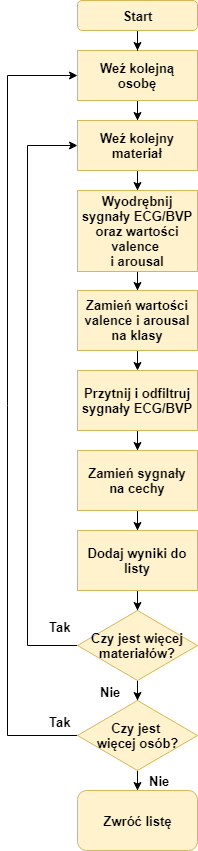
\includegraphics[width=0.25\linewidth]{images/preprocessing_flow.png}
	\caption{Schemat przedstawiający proces przetworzenia danych do zbioru uczącego}
	\label{fig:preprocessing_flow}
\end{figure}

Mając identyfikator osoby i~eksperymentu, z~wczytanych danych zostały wyodrębnione sygnały z~elektrokardiogramu a~w przypadku zbioru DEAP z~odczytów pulsu objętości krwi. Zostały także odczytane wartości \textit{valence} i~\textit{arousal}, na podstawie których określony zostanie cel przygotowywanego modelu. Aby ujednolicić otrzymane wartości ocen, przeskalowano je do zakresu od 1~do 9, a~następnie zamieniono na 9~klas, odpowiadających połączeniu 3~poziomów wartości dla każdej z~ocen, tak jak pokazano to na rysunku~\ref{fig:model_classes}. Taki podział pozwoli na objęcie stanów emocjonalnych charakteryzujących się niską lub wysoką wartością każdej z~ocen, uwzględniając jednocześnie wartości środkowe opisujące stan neutralny. Kolejnym krokiem było dostosowanie sygnałów do przetworzenia ich na cechy. Ponieważ reakcje fizjologiczne, które mogłyby wskazać na zmianę odczuwanej emocji, następują dopiero po jakimś czasie, wczytane dane zostały obcięte do ostatnich 50~sekund eksperymentu. Następnie, aby pozbyć się ewentualnych szumów i~wygładzić przebieg sygnałów, przefiltrowano je przy pomocy pasmowoprzepustowego filtru Butterwortha. Częstotliwości graniczne zostały dobrane na podstawie artykułu Fedotova~\cite{fedotov_optimal_cutoff_2016} poświęconego określeniu optymalnych wartości tych parametrów podczas filtrowania sygnału z~elektrokardiogramu.
\begin{figure}
	\centering
	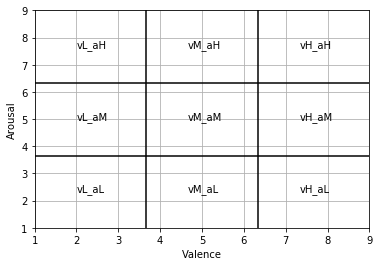
\includegraphics[width=0.5\linewidth]{images/model_classes.png}
	\caption{Podział ocen \textit{valence} i~\textit{arousal} na 9~klas}
	\label{fig:model_classes}
\end{figure}

Tak przygotowany sygnał został następnie wykorzystany do obliczenia cech, które będą wykorzystane w~przygotowywanym modelu. Na początku z~odczytanów sygnałów wyciągnięte zostały interwały pomiędzy kolejnymi uderzeniami serca. Aby określić te wartości, w~przypadku sygnału z~elektrokardiogramu należało znaleźć położenia kolejnym załamków R, natomiast dla pomiarów pulsu objętości krwi kolejne powtórzenia danej fazy pracy serca. Do wykrycia tych punktów wykorzystana biblioteka PeakUtils\footnote{\url{https://scikit-learn.org/}} oferująca algorytm do wykrywania wierzchołków w~podanym sygnale. Wymagany parametr minimalnej odległości pomiędzy kolejnych wierzchołkami był wyliczany na podstawie wzoru:
$$
\frac{60*f}{max_{hr}}
$$
gdzie $f$ oznaczało częstotliwość danych zbioru, z~którego pochodziła próbka sygnału, a~$max_{hr}$ przyjętą najwyższą możliwą wartość tętna. Eksperymentalnie została ona ustawiona na 135~uderzeń serca na minutę. Mając na uwadze fakt, że biblioteka mogła wykryć także nieprawidłowe położenia wierzchołków, po wyznaczeniu interwałów przefiltrowano je, odrzucając wartości znacznie odbiegające od mediany z~odczytów. Na podstawie odfiltrowanych wartości zostały obliczone ilości uderzeń serca na minutę, a~następnie zostały określone następujące cechy statystyczne, które będą brane pod uwagę podczas uczenia modelu:
\begin{itemize}
	\item Minimalna i~maksymalna ilość uderzeń serca na minutę
	\item Średnia wartość tętna i~interwałów między uderzeniami
	\item Odchylenie standardowe tętna
	\item Kurtoza tętna i~interwałów -- opisuje, jak bardzo wyniki są skoncentrowane lub oddalone od średniej
	\item Współczynnik skośności dla tętna i~interwałów -- opisuje, jak dane rozkładają się wokół średniej.
	\item Procentowa ilość odczytów tętna i~interwałów powyżej wartości: $\text{średnia pomiaru} + \text{odchylenie standardowe}$
	\item Procentowa ilość odczytów  tętna i~interwałów poniżej wartości: $\text{średnia pomiaru} - \text{odchylenie standardowe}$
	\item Średnie odchylenie bezwględne (MAD) dla wartości interwałów pomiędzy uderzeniami serca
\end{itemize}

Analizie została poddana także zmienność rytmu zatokowego, którą rozpatrzono jako parametry opisujące ją w~trzech dziedzinach. Pierwszą z~nich jest dziedzina czasu, w~ramach której można określić następujące parametry:
\begin{itemize}
	\item odchylenie standardowe interwałów pomiędzy kolejnymi uderzeniami (SDNN)
	\item średnia kwadratowa różnic pomiędzy kolejnymi interwałami (RMSSD)
	\item odchylenie standardowe różnic między kolejnymi interwałami (SDSD)
	\item procentowa ilość interwałów, które różnią się od poprzedniego interwału o~więcej niż 20~ms (pNN20)
	\item procentowa ilość interwałów, które różnią się od poprzedniego interwału o~więcej niż 50~ms (pNN50)
\end{itemize}
Kolejną z~dziedzin, w~ramach której rozpatrywana jest zmienność rytmu zatokowego, jest częstotliwość. 
Parametry w~ramach tej dziedziny zostały określone poprzez wygenerowanie periodogramu za pomocą metody Welcha~\cite{welch_1967} dostępnej jako funkcja w~bibliotece SciPy, a~następnie wyznaczeniu mocy widma w~zakresie określonych częstotliwości~\cite{hrv_overwiev_2017}:
\begin{itemize}
	\item 0.04--0.15 Hz -- zakres LF, dostarczający informacji o~krótkich zmianach w~tętnie
	\item 0.15--0.4 Hz -- zakres HF, dostarczający informacji o~zmianach związanych z~cyklem oddechowym
\end{itemize}
Jako dodatkowy parametr wykorzystano także stosunek mocy sygnałów LF do HF. Wysoka wartość tej cechy jest widoczna w~sytuacjach polegających na walce lub ucieczce, natomiast wartości niskie w~przypadku zachowań pozytywnych, takich jak zawarcie przyjaźni.

Trzecią dziedziną, w~ramach której można przeprowadzić analizę zmienności rytmu zatokowego, jest dziedzina nieliniowa. W~ramach analizy wyznaczany jest wykres Poincaré, który przedstawia korelację pomiędzy kolejnymi interwałami. Oznacza to, że współrzędne każdego z~punktów wykresu są opisane jako sąsiadujące wartości interwałów pomiędzy kolejnymi uderzeniami. Cechy wyznaczane w~ramach tej analizy to mała i~duża oś elipsy okalającej wszystkie punkty wykresu. Mała oś (SD1) jest to odchylenie standardowe odległości punktów od osi $y=x$ i~opisuje krótkoczasową zmienność rytmu serca. Duża oś natomiast odpowiada odchyleniu standardowemu odległości każdego z~punktów od osi $y=x+avg$, gdzie $avg$ oznacza średnią wartość interwałów. Wartości z~tej osi opisują długoczasową zmienność rytmu serca. Jako dodatkową cechę wykorzystano także stosunek SD1 do SD2.

Dla każdego eksperymentu wyciągnięciu wszystkich z~wyżej opisanych cech połączono je z~wcześniej wyznaczoną klasą i~dodano do zbioru uczącego. Przygotowany zbiór następnie przefiltrowano, usuwając te przypadki, w~których brakowało przynajmniej jednej cechy. Ze względu na działania wykonywane podczas uczenia i~dopracowywania modelu, cechy nie zostały znormalizowane na etapie przetwarzania danych.

\section{Wybór modelu}
%Ewaluacja w~hyperopt, statystyki skuteczności, ostateczny wybór modelu
Do uczenia modelu na podstawie przygotowanego zbioru danych uczących zostały wykorzystane następujące klasyfikatory z~biblioteki scikit-learn\footnote{\url{https://scikit-learn.org/}}:
\begin{itemize}
	\item RandomForestClassifier
	\item ExtraTreesClassifier
	\item SupportVectorClassifier (SVC)
	\item KNeighborsClassifier
	\item GradientBoostingClassifier
\end{itemize}

W pierwszej iteracji wszystkie modele były uczone dla domyślnych wartości parametrów. Następnie, aby sprawdzić czy skuteczności tak przygotowanych modeli są wiarygodne dla danych spoza zbioru uczącego, przeprowadzono \textit{K}-krotną walidację krzyżową. Metoda ta polega na podzieleniu zbioru na \textit{K} podzbiorów, które następnie są wykorzystane do przeprowadzenia \textit{K} iteracji uczenia modelu, gdzie jako dane uczące wybieranych jest \textit{K}-1 podzbiorów, natomiast ostatni jest wykorzystywany jako dane testowe. W~wyniku przeprowadzenia walidacji zostaje wygenerowanych \textit{K} modeli o~określonych skutecznościach, które następnie można wykorzystać do obliczenia średniej skuteczności modelu. W~obu przypadkach cechy ostały poddane standaryzacji. Wartości procentowe skuteczności zarówno dla przypadku domyślnego, jak i~walidacji krzyżowej przedstawia tabela~\ref{tab:models_accuracies}.

\begin{table}
	\centering
	\caption{Skuteczności wybranych modeli przy określonych parametrach}
	\label{tab:models_accuracies}
	\begin{tabular}{|l|l|l|l|}
		\hline
		\textbf{Algorytm} & \textbf{\begin{tabular}[c]{@{}l@{}}Skuteczność\\ dla domyślnych\\ parametrów\end{tabular}} & \textbf{\begin{tabular}[c]{@{}l@{}}Skuteczność\\ po przeprowadzeniu\\ walidacji krzyżowej\end{tabular}} & \textbf{\begin{tabular}[c]{@{}l@{}}Skuteczność\\ po  optymalizacji\\ parametrów\end{tabular}} \\ \hline
		RandomForestClassifier      & 28\%                 & 27\%                                                                                                  & 35\%                                                                                        \\ \hline
		ExtraTreesClassifier        & 31\%                 & 29\%                                                                                                  & 36\%                                                                                        \\ \hline
		SVC               & 25\%                 & 25\%                                                                                                  & 28\%                                                                                        \\ \hline
		GradientBoostingClassifier               & 24\%                 & 24\%                                                                                                  & -                                                                                         \\ \hline
		KNeighboursClassifier               & 21\%                 & 24\%                                                                                                  & -                                                                                       \\ \hline
	\end{tabular}
\end{table}

Aby osiągnąć większą skuteczność, należało przeprowadzić optymalizację parametrów. Zdecydowano się ją wykonać jedynie dla tych modeli, które wykazywały skuteczność wyższą lub równą 25\%. Wykorzystana została do tego biblioteka hyperopt-sklearn\footnote{\url{http://hyperopt.github.io/hyperopt-sklearn/}}, która pozwala na odszukanie jak najlepszych parametrów modelu w~zależności od zadanych danych wejściowych. Funkcja estymująca na wejściu przyjmuje model, dla którego chcemy znaleźć parametry, sposób normalizacji cech, liczbę konfiguracji, dla których ma zostać przeprowadzona analiza oraz maksymalny czas, w~jakim każda z~prób powinna się zakończyć. Dla każdego z~modeli liczba prób została ustalona na 100, natomiast maksymalny czas dla prób ustawiony został na 5~minut. Parametr odpowiadający za normalizację cech został ustawiony na wartość dowolną, dzięki czemu estymator będzie mógł także znaleźć funkcję normalizującą cechy wraz z~jej parametrami, która w~połączeniu ze znalezionymi parametrami modelu da najlepsze wyniki. Skuteczności modeli po optymalizacji ich parametrów oraz funkcji do normalizacji cech przedstawione zostały w~ostatniej kolumnie tabeli~\ref{tab:models_accuracies}. Największy przyrost, a~jednocześnie najwyższą wartość skuteczności wynoszącą 36\% można zauważyć dla klasyfikatora wykorzystujące ekstremalne drzewa ekstremalnie losowe. Dla tego modelu została ponownie przeprowadzona optymalizacja parametrów, tym razem dla dłuższego czasu maksymalnego i~liczby prób równej 1200, jednak wynik poprawił się zaledwie o~1\%. 

Taka skuteczność nie pozwala na pewne rozpoznawanie emocji na podstawie odczytów samej pracy serca. Głównym powodem może być tutaj fakt, że czas, na podstawie którego wykrywane były emocje, był na tyle długi, że w~trakcie badania użytkownicy mogli odczuwać więcej niż jedną emocję. Ponieważ nie jest jeszcze obecnie możliwe powiązanie wzorców zmian w~reakcjach fizjologicznych z~konkretnymi emocjami przy pomocy wzorów, nie było także możliwości wyboru odpowiednich fragmentów sygnałów w~zależności od eksperymentu. Możliwe, że dołączenie do analizy sygnałów na temat reakcji elektrodermalnej, czy odczytów z~elektroencefalogramu pozwoliłoby na uzyskanie wyższej skuteczności, jednak wykorzystanie sensorów do pomiarów tych sygnałów mogłoby wprowadzić wysoki dyskomfort podczas użytkowania, co kolidowałoby z~wymaganiami architektury sprzętowej przygotowywanego interfejsu. Skuteczność rozpoznawania emocji przy pomocy wybranego modelu może zostać poprawiona dzięki odczytom z~akcelerometru wbudowanego w~kontroler. Ostateczny sposób wyliczania i~interpretacja stanów emocjonalnych na podstawie przygotowanego modelu oraz pomiarów z~akcelerometru zostanie opisana w~rozdziale~\ref{cha:implementacja}.